\documentclass[11pt, oneside]{article}   	% use "amsart" instead of "article" for AMSLaTeX format
\usepackage{geometry}                		% See geometry.pdf to learn the layout options. There are lots.
\geometry{letterpaper}                   		% ... or a4paper or a5paper or ... 
%\geometry{landscape}                		% Activate for rotated page geometry
%\usepackage[parfill]{parskip}    		% Activate to begin paragraphs with an empty line rather than an indent
\usepackage{graphicx}				% Use pdf, png, jpg, or eps§ with pdflatex; use eps in DVI mode
								% TeX will automatically convert eps --> pdf in pdflatex		
\usepackage{amssymb,amsmath}
\usepackage{amsthm}
\usepackage{float}
\usepackage{bm}

\usepackage{ragged2e}
\usepackage{adjustbox}
\usepackage{blindtext}
\usepackage{listings}
\usepackage[utf8]{inputenc}
\newcommand{\Var}{\operatorname{Var}}
\newcommand{\E}{\operatorname{E}}
\newcommand{\Cov}{\operatorname{Cov}}
% Default fixed font does not support bold face
\DeclareFixedFont{\ttb}{T1}{txtt}{bx}{n}{12} % for bold
\DeclareFixedFont{\ttm}{T1}{txtt}{m}{n}{12}  % for normal


\usepackage{scalerel,stackengine}
\stackMath
\newcommand\reallywidehat[1]{%
\savestack{\tmpbox}{\stretchto{%
  \scaleto{%
    \scalerel*[\widthof{\ensuremath{#1}}]{\kern-.6pt\bigwedge\kern-.6pt}%
    {\rule[-\textheight/2]{1ex}{\textheight}}%WIDTH-LIMITED BIG WEDGE
  }{\textheight}% 
}{0.5ex}}%
\stackon[1pt]{#1}{\tmpbox}%
}
\parskip 1ex


\lstset{language=R,
    basicstyle=\small\ttfamily,
    stringstyle=\color{DarkGreen},
    otherkeywords={0,1,2,3,4,5,6,7,8,9},
    morekeywords={TRUE,FALSE},
    deletekeywords={data,frame,length,as,character},
    keywordstyle=\color{blue},
    commentstyle=\color{DarkGreen},
     %frame=single, % adds a frame around the code
     backgroundcolor=\color{lightgray},
}
\usepackage[svgnames]{xcolor}
\title{STAT211 Mandatory Homework 8}
\author{Yapi Donatien Achou}
%\date{}							% Activate to display a given date or no date

\begin{document}

\maketitle 
\tableofcontents
\newpage
 
 \section{Problem 8.1}
 \subsection{Part a}
 \begin{lstlisting}
yearlySunsplts <- na.omit(read.table(file="data/yearly_sunspots.txt",header=TRUE))
dat <- yearlySunsplts$sunspots
png("yearly.png")
plot(dat,col="blue",type="b")
 \end{lstlisting}
 \begin{figure}[H] %  figure placement: here, top, bottom, or page
    \centering
    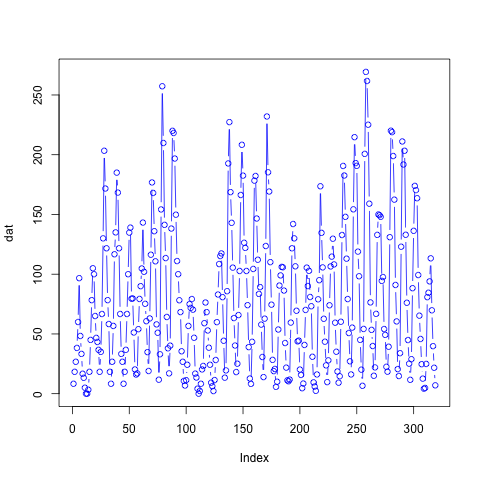
\includegraphics[width=4in]{yearly.png} 
    \caption{Yearly sunspot}
    \label{fig:example}
 \end{figure}
 
 \clearpage
 \subsection{Part b}
 Let 
 \begin{equation}
 Y_{t} = X_{t} - \bar{X}_{t}
 \end{equation}
 \begin{figure}[H] %  figure placement: here, top, bottom, or page
    \centering
    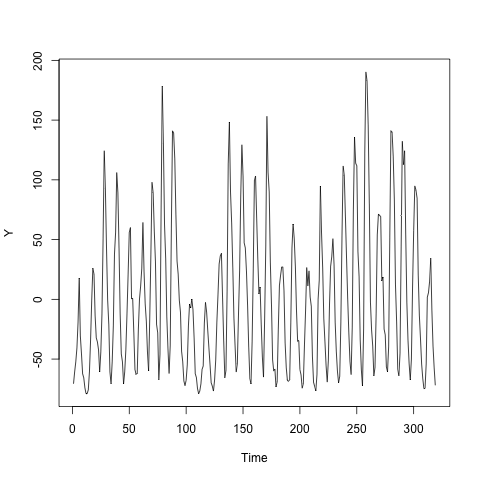
\includegraphics[width=4in]{y.png} 
    \caption{Plot of $ Y_{t} = X_{t} - \bar{X}_{t}$}
    \label{fig:y}
 \end{figure}
 \justify
 Figure \ref{fig:y} shows the plot of $ Y_{t} = X_{t} - \bar{X}_{t}$.
 
 
 \begin{lstlisting}
yearlySunsplts <- na.omit(read.table(file="data/yearly_sunspots.txt",header=TRUE))
X <- yearlySunsplts$sunspots
Y <- X-mean(X)
png("note/acf.png")
acf(Y,col="blue")
 \end{lstlisting}
 
  
 \begin{figure}[H] %  figure placement: here, top, bottom, or page
    \centering
    
\includegraphics[width=4in]{acf.png} 
    \caption{ACF}
    \label{fig:acf}
 \end{figure}
 
 \begin{lstlisting}
yearlySunsplts <- na.omit(read.table(file="data/yearly_sunspots.txt",header=TRUE))
X <- yearlySunsplts$sunspots
Y <- X-mean(X)
png("note/pacf.png")
pacf(Y,col="blue")
 \end{lstlisting}
 

 \begin{figure}[H] %  figure placement: here, top, bottom, or page
    \centering
    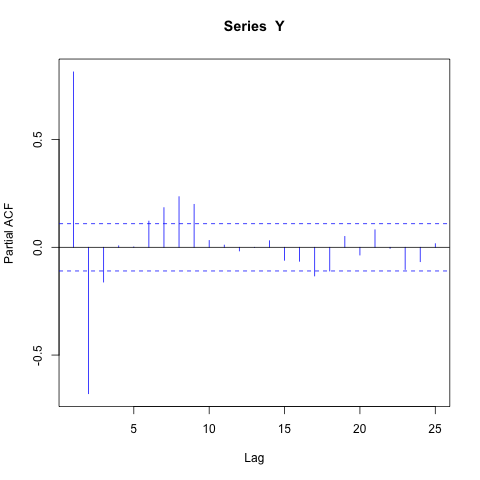
\includegraphics[width=4in]{pacf.png} 
    \caption{PACF}
    \label{fig:pacf}
 \end{figure}

 
 \subsection{Part c: Fit AR(2) model}
 \begin{lstlisting}
yearlySunsplts <- na.omit(read.table(file="data/yearly_sunspots.txt",header=TRUE))
X <- yearlySunsplts$sunspots
Y <- X-mean(X)
ar2 <- ar(Y,order.max=2)
print(ar2)

Call:
ar(x = Y, order.max = 2)

Coefficients:
      1        2  
 1.3666  -0.6792  

Order selected 2  sigma^2 estimated as  704.1
 \end{lstlisting}
 From the simulation result $\hat{\phi}_{1} = 1.3666, \hat{\phi}_{1} =0.6792, \sigma_{2} = 704.1$
 \begin{figure}[H] %  figure placement: here, top, bottom, or page
    \centering
    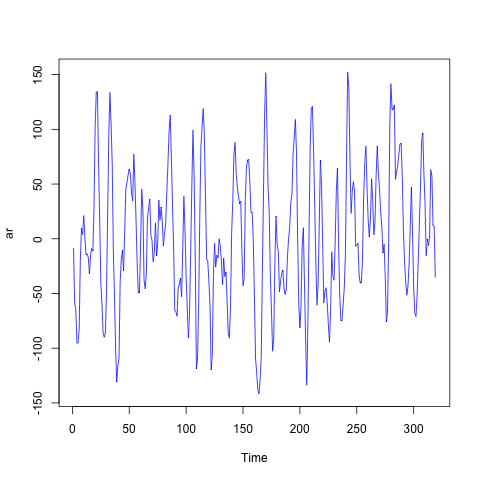
\includegraphics[width=4in]{ar.png} 
    \caption{The simulated AR(2) process}
    \label{fig:ar2}
 \end{figure}
 
 \subsection{Part d: Periodogram}
 \begin{lstlisting}
library(TSA)
set.seed(10)
yearlySunsplts <- na.omit(read.table(file="data/yearly_sunspots.txt",header=TRUE))
X <- yearlySunsplts$sunspots
Y <- X-mean(X)
m <- length(Y)
ar.sim <- arima.sim(model=list(ar=c(1.3666, -0.6792)),n=m)
per <- periodogram(ar.sim)
spectrum <- per$spec
png("periodogram.png")
plot(spectrum,col="blue",type="b")
 \end{lstlisting}
\begin{figure}[H] %  figure placement: here, top, bottom, or page
   \centering
   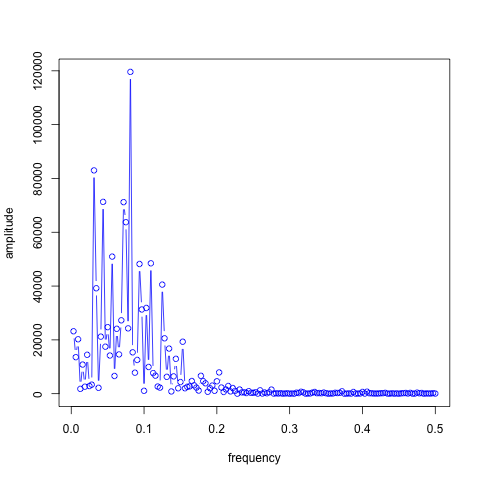
\includegraphics[width=4in]{periodogram.png} 
   \caption{Periodogram}
   \label{fig:per}
\end{figure}


\subsection{Part d: Smooth periodogram}
 \begin{lstlisting}
library(TSA)
set.seed(10)
yearlySunsplts <- na.omit(read.table(file="data/yearly_sunspots.txt",header=TRUE))
X <- yearlySunsplts$sunspots
Y <- X-mean(X)
m <- length(Y)
ar.sim <- arima.sim(model=list(ar=c(1.3666, -0.6792)),n=m)
per <- periodogram(ar.sim)
amplitude <- per$spec
smoothPeriodogram = filter(amplitude, filter = c(1/3,3), sides=2)
png("smoothPeriodogram.png")
plot(smoothPeriodogram,col="blue",type="b")
 \end{lstlisting}
\begin{figure}[H] %  figure placement: here, top, bottom, or page
   \centering
   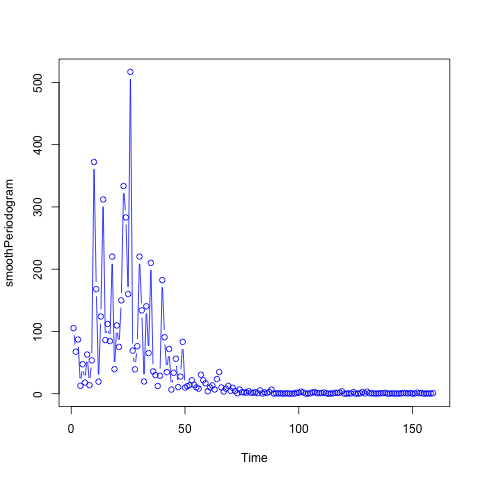
\includegraphics[width=4in]{smoothPeriodogram.png} 
   \caption{Smoother periodogram}
   \label{fig:per}
\end{figure}


\subsection{Part f: Spectral density}
\begin{lstlisting}
library(TSA)
set.seed(10)
yearlySunsplts <- na.omit(read.table(file="data/yearly_sunspots.txt",header=TRUE))
X <- yearlySunsplts$sunspots
Y <- X-mean(X)
m <- length(Y)
ar.sim <- arima.sim(model=list(ar=c(1.3666, -0.6792)),n=m)
spectralDensity <- spectrum(ar.sim,method="ar")
png("spectralDensity.png")
plot(spectralDensity,col="blue")
 \end{lstlisting}
\begin{figure}[H] %  figure placement: here, top, bottom, or page
   \centering
   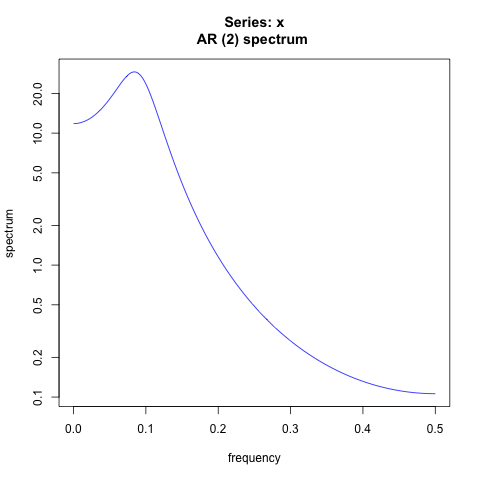
\includegraphics[width=4in]{spectralDensity} 
   \caption{Spectral density}
   \label{fig:per}
\end{figure}

 \subsection{Part g}
 \begin{figure}[H] %  figure placement: here, top, bottom, or page
    \centering
    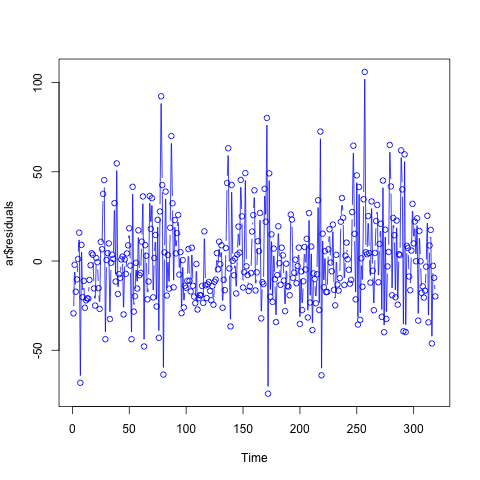
\includegraphics[width=4in]{residual.png} 
    \caption{Residual}
    \label{fig:res}
 \end{figure}
 
 \begin{figure}[H] %  figure placement: here, top, bottom, or page
    \centering
    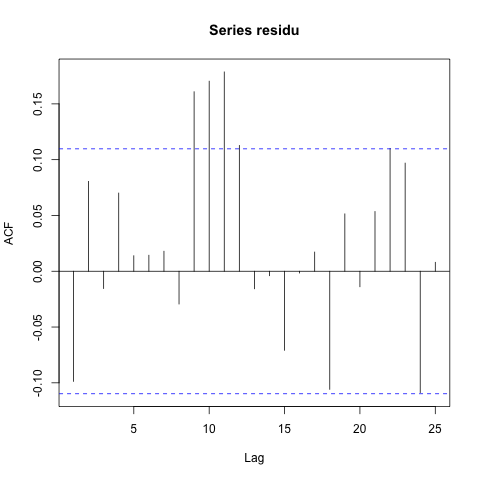
\includegraphics[width=4in]{acfresidual.png} 
    \caption{ACF of Residual}
    \label{fig:acfres}
 \end{figure}
 
 \begin{figure}[H] %  figure placement: here, top, bottom, or page
    \centering
    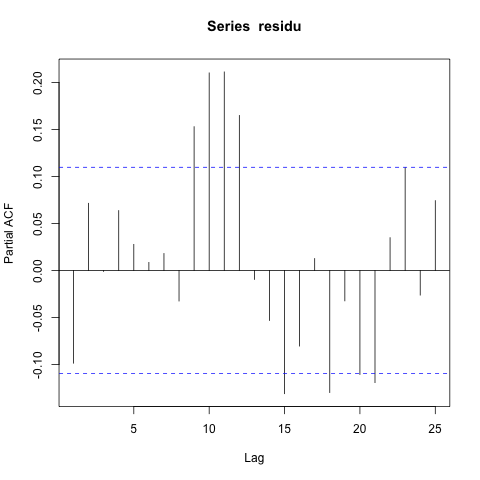
\includegraphics[width=4in]{pacfresidual.png} 
    \caption{PACF of Residual}
    \label{fig:pacfres}
 \end{figure}
 
 \subsection{Part h}
 \begin{figure}[H] %  figure placement: here, top, bottom, or page
    \centering
    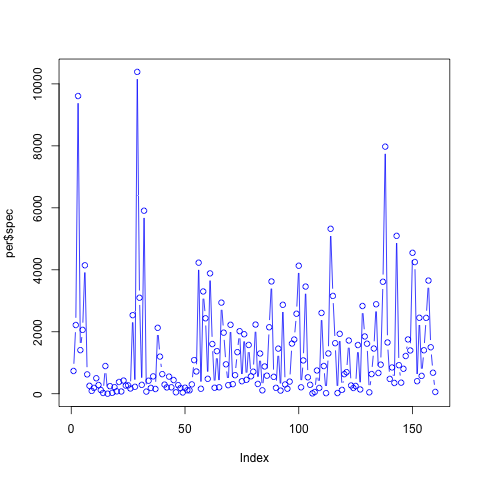
\includegraphics[width=2in]{residualPer.png} 
    \caption{Periodogram of residual}
    \label{fig:resper}
 \end{figure}
 
  \begin{figure}[H] %  figure placement: here, top, bottom, or page
    \centering
    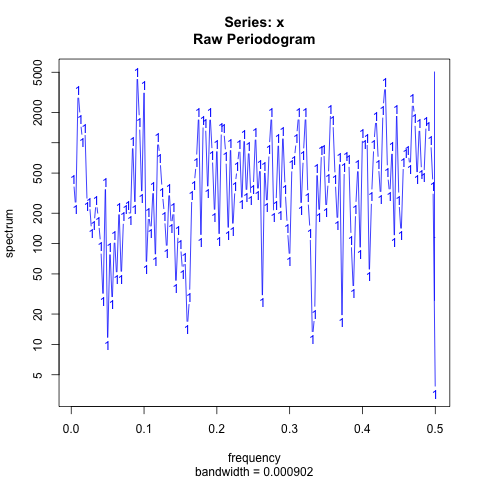
\includegraphics[width=2in]{residualSpec.png} 
    \caption{Spectral density of residual}
    \label{fig:specr}
 \end{figure}
 
 
 \section{Problem 8.2}
 In this exercise we study the spectral representation of a time series. The spectral representation of a time series is used to decompose a time series into sums of sinusoidal components \cite{petter}. By doing so, we can identify the dominant periods or frequencies of a time series by using its periodogram \cite{penn}. The periodogram is a sample based function that gives an estimate of the spectral density \cite{petter}. If $f(\cdot)$ is the spectral density and $I_{n}(\cdot)$ is the periodogram of $n$ observations, then $I_{n}(\cdot)$ can be view as an estimation of $2\pi f(\cdot)$ \cite{petter}.
\justify 
The spectral density for an AR(2) model is given by 
 \begin{equation}
 \begin{split}
 f(w) &= \frac{\sigma^{2}}{2\pi} \frac{1}{| \phi(\exp(-iw))|^{2}}, \quad w \in (-\pi, \pi], \quad \phi(z) = 1-\phi_{1}z - \phi_{2}z^{2}.\\
        &=\frac{\sigma^{2}}{2\pi} \frac{1}{|1-\phi_{1}e^{-iw} - \phi_{2}e^{-2iw} |^{2}}
 \end{split}
 \end{equation}
 The spectral density of a stationary process $\{X_{t}\}$ specifies the frequency decomposition of the autocovariance function (ACF) \cite{petter}.
 \subsection{Part a: Spectral density}
 \begin{lstlisting}
f <- function(w){
  phi1 <- 1.4
  phi2 <- -0.9
  phi <- 1-phi1*w-phi2*w**2
  sigma <- 1
  denominator <- abs(1-phi1*exp(-(0+1i)*w) - phi2*exp(-(0+2i)*w))**2
  factor <- (sigma*sigma)/(2*pi)
  value <- factor*(1./denominator)
  return(value)

}
set.seed(10)
w <- seq(-pi, pi)
png("theoreticalDensity.png")
plot(f(w), col="blue",type="b",xlab="frequency")
\end{lstlisting}

\begin{figure}[H] %  figure placement: here, top, bottom, or page
   \centering
   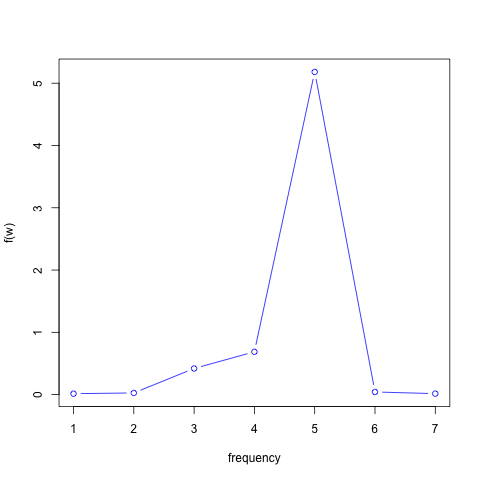
\includegraphics[width=3in]{../code/theoreticalDensity.png} 
   \caption{Spectral density of the AR(2) process}
   \label{fig:sd}
\end{figure}

\subsection{Part b: Comparing spectral density}
For spectral for $\phi_{2}=0.95$
 \begin{lstlisting}
f <- function(w){
  phi1 <- 1.4
  phi2 <- 0.95
  phi <- 1-phi1*w-phi2*w**2
  sigma <- 1
  denominator <- abs(1-phi1*exp(-(0+1i)*w) - phi2*exp(-(0+2i)*w))**2
  factor <- (sigma*sigma)/(2*pi)
  value <- factor*(1./denominator)
  return(value)

}
set.seed(10)
w <- seq(-pi, pi)
png("theoreticalDensity.png")
plot(f(w), col="blue",type="b",xlab="frequency")
\end{lstlisting}


\begin{figure}[H] %  figure placement: here, top, bottom, or page
   \centering
    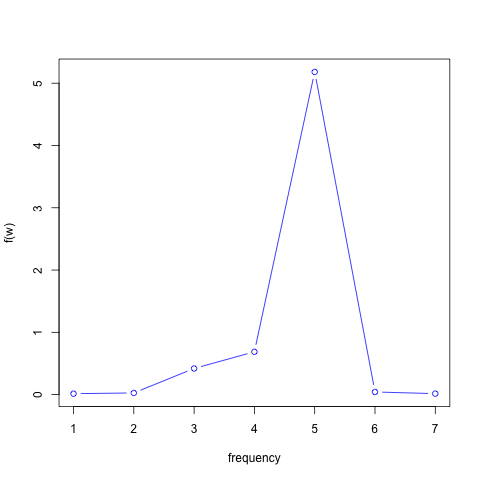
\includegraphics[width=2.5in]{../code/theoreticalDensity.png}
   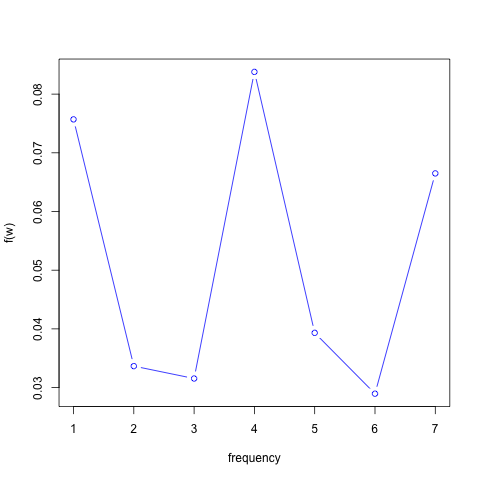
\includegraphics[width=2.5in]{../code/theoreticalDensity2.png} 
   \caption{Spectral density of the AR(2) process. Left $\phi_{2} = -0.90$, right $\phi_{2} = 0.95$ }
   \label{fig:sd2}
\end{figure}

We can observe from Figure (\ref{fig:sd2}) that the spectral density for $\phi_{2} = 0.95$ oscillate more compared to the one with $\phi_{2} = -0.9$.
%\begin{proof}
%We know that
%
%\end{proof}

\subsection{Part c: Simulation of the AR(2) process}
Simlating the AR(2) process with 100 obervations
\begin{lstlisting}
# Plot of AR(2) model
ar.sim <- arima.sim(model=list(ar=c(1.4, -0.9)), n=100)
ts.plot(ar.sim)
\end{lstlisting}
\begin{figure}[H] %  figure placement: here, top, bottom, or page
   \centering
   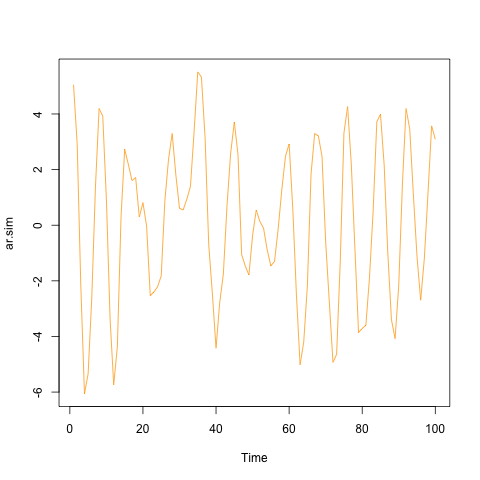
\includegraphics[width=2.5in]{../code/armaSimulation1.png} 
   \caption{AR(2) simulation for $\phi_{1} = 1.4, \phi_{2}= -0.9$}
   \label{fig:arma}
\end{figure}
\begin{lstlisting}
#Periodogram  of AR(2) model
ar.sim <- arima.sim(model=list(ar=c(1.4, -0.9)), n=100)
per <- periodogram(ar.sim)
plot(per)
\end{lstlisting}
\begin{figure}[H] %  figure placement: here, top, bottom, or page
   \centering
   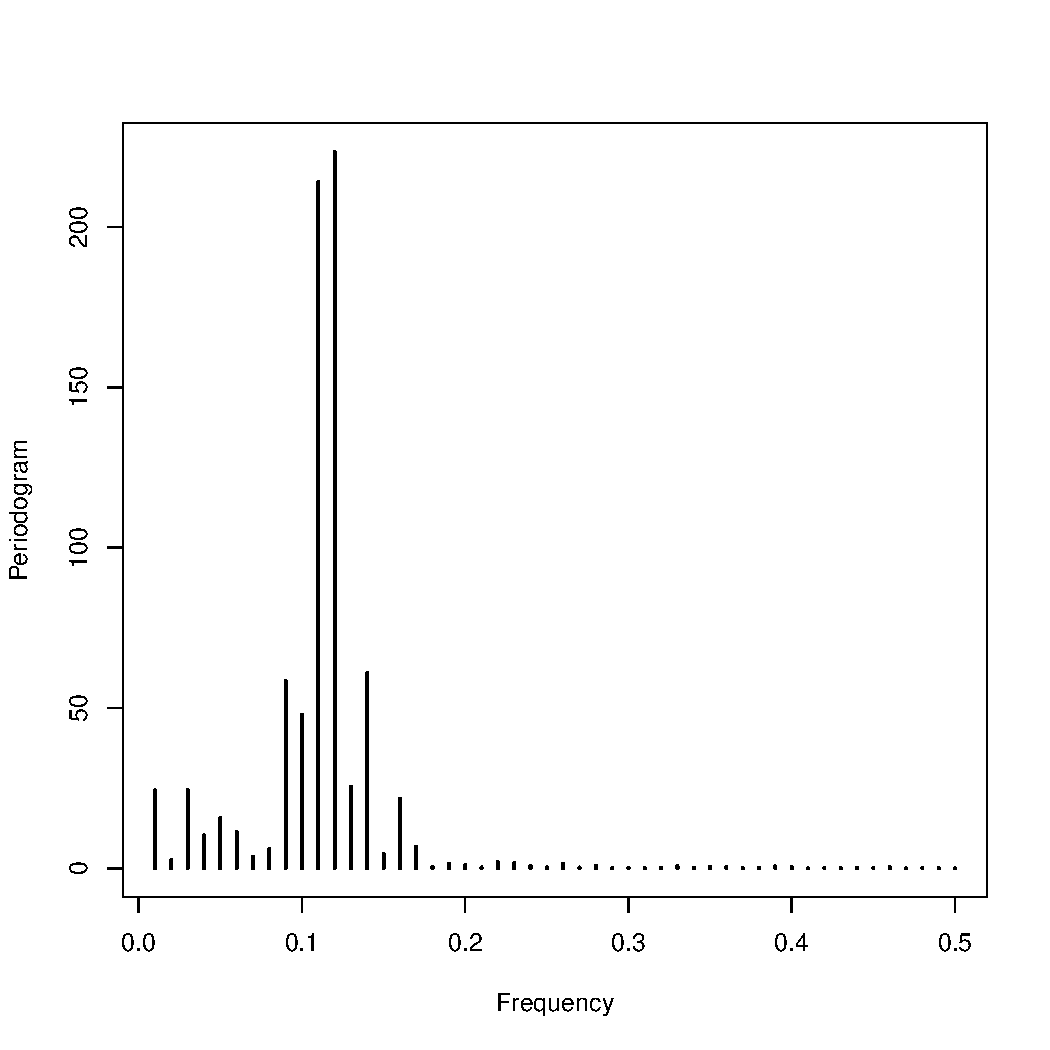
\includegraphics[width=2in]{../code/periodogram1.pdf} 
    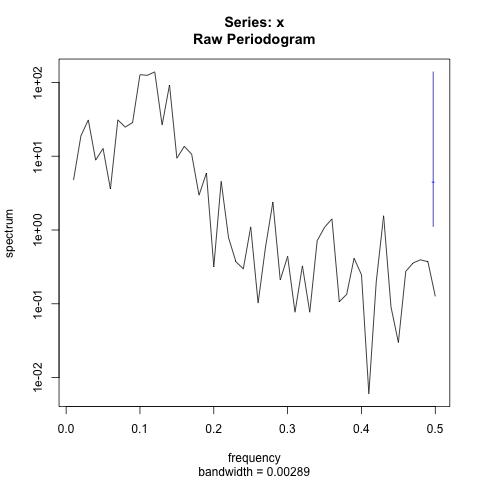
\includegraphics[width=2in]{../code/periodogram.png} 
   \caption{Periodogram of the AR(2) process}
   \label{fig:per}
\end{figure}

\begin{lstlisting}
#Moving average smoothening of periodogram
set.seed(10)
ar.sim <- arima.sim(model=list(ar=c(1.4, -0.9)), n=100)
periodogram <- periodogram(ar.sim)
spectrum <- periodogram$spec
trendpattern = filter(spectrum, filter = c(1/3,3), sides=2)
plot(trendpattern)
\end{lstlisting}
\begin{figure}[H] %  figure placement: here, top, bottom, or page
   \centering
   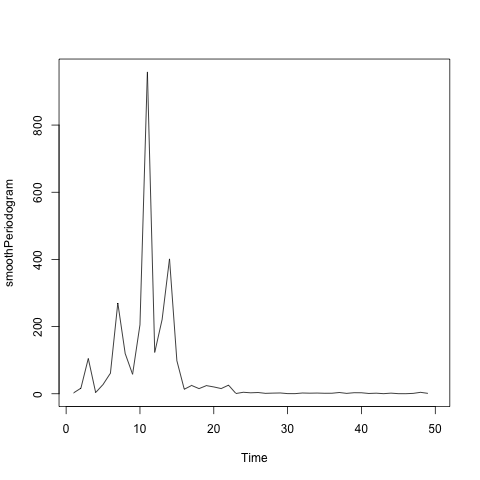
\includegraphics[width=4in]{../code/smoonth.png} 
   \caption{Smooth periodogram}
   \label{fig:sm}
\end{figure}
\begin{lstlisting}
#Estimated spectral density
set.seed(10)
ar.sim <- arima.sim(model=list(ar=c(1.4, -0.9)), n=100)
estimatedSpecralDensity <- spectrum(ar.sim,method="ar")
png("EstimatedSpectralDensity.png")
plot(estimatedSpecralDensity)
\end{lstlisting}

\begin{figure}[H] %  figure placement: here, top, bottom, or page
   \centering
   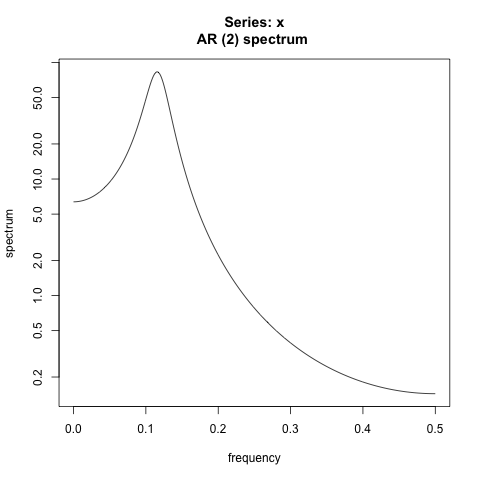
\includegraphics[width=4in]{../code/EstimatedSpectralDensity.png} 
   \caption{Estimated spectral density from R function spectrum}
   \label{fig:es}
\end{figure}
\justify
Figure \ref{fig:arma} shows the simulated AR(2) process, Figure \ref{fig:per} shows the periodogram of the AR(2) process, Figure \ref{fig:sm} shows the smoothen periodogram and Figure \ref{fig:es} shows the
estimated spectral density from the AR(2) model.


\clearpage
\subsection{Part d}
Recall the plot of the AR(2) model
\begin{figure}[H] %  figure placement: here, top, bottom, or page
   \centering
   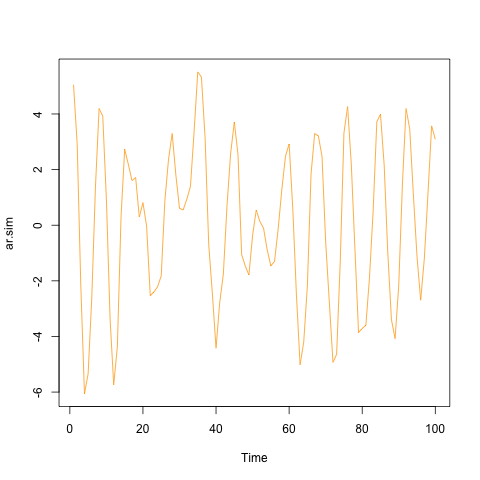
\includegraphics[width=2.5in]{../code/armaSimulation1.png} 
   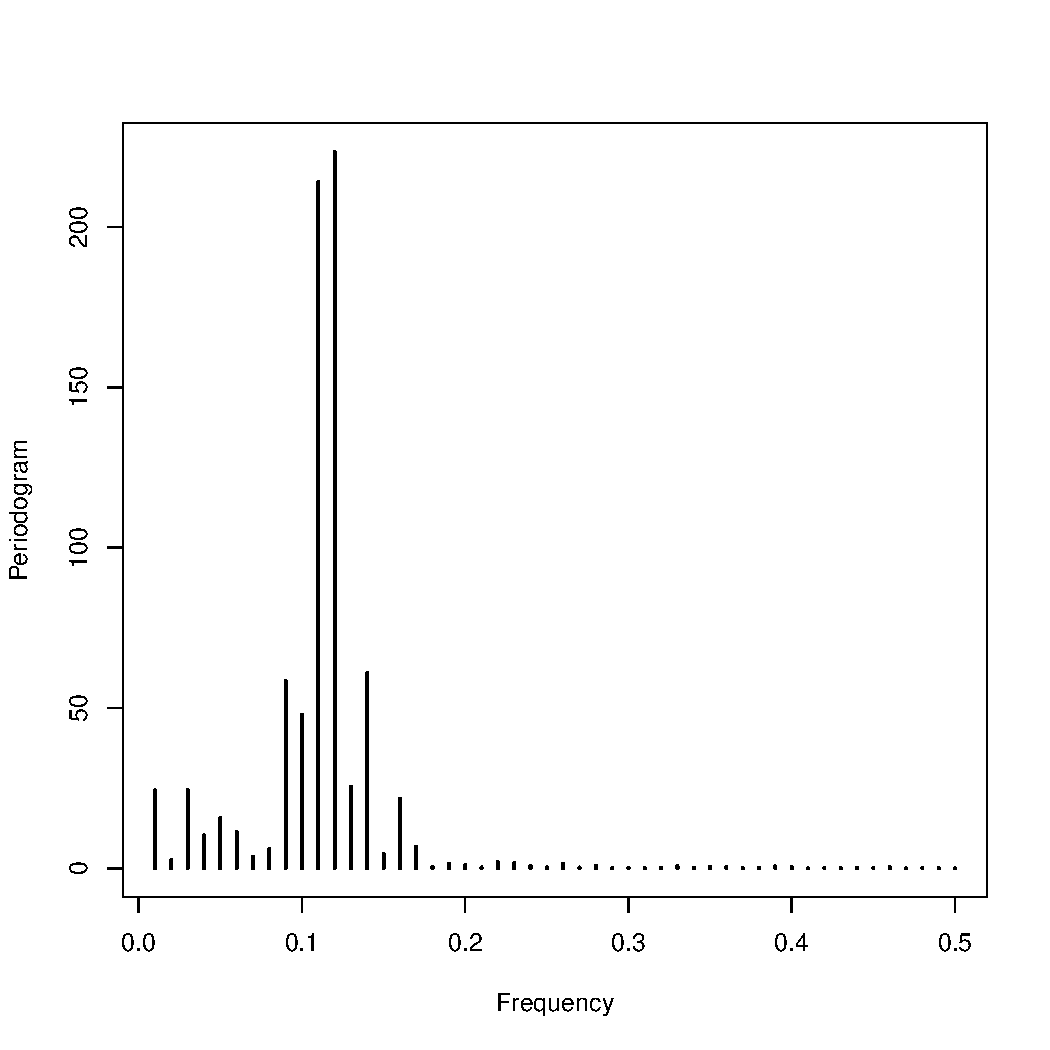
\includegraphics[width=2.5in]{../code/periodogram1} 
   \caption{AR(2) simulation for $\phi_{1} = 1.4, \phi_{2}= -0.9$ left and periodogram right}
   \label{fig:ar2}
\end{figure}
\justify
From Figure \ref{fig:ar2} we can clearly see a periodic structure of the time series modelled by the AR(2) process. From the periodogram, we can see a pick. We get the peak and corresponding frequency as follow
\begin{lstlisting}
ar.sim <- arima.sim(model=list(ar=c(1.4, -0.9)), n=100)
periodogram <- periodogram(ar.sim)
spectrum <- periodogram$spec
frequency <- periodogram$freq
pick <- max(spectrum)
pickIndex = match(pick, spectrum)
freq <- frequency[pickIndex]
print(pick)
print(freq)

>>[1] 315.5908
>>[1] 0.11
\end{lstlisting}
\justify
We observe a peak at a frequency of 0.11 which corresponds to period 
\begin{equation}
T = \frac{1}{0.11} = 9
\end{equation} 
which means that a cycle is completed in 9 time periods.


\subsection{Part e}
Simulation with 1000 observation

\begin{figure}[H] %  figure placement: here, top, bottom, or page
   \centering
   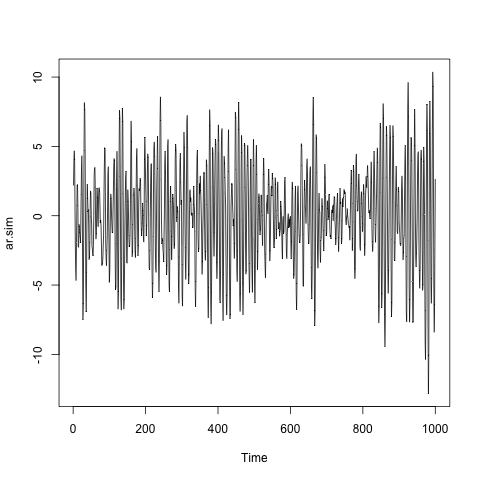
\includegraphics[width=4in]{../code/simulation1000.png} 
   \caption{Simulation with 1000 obervartion}
   \label{fig:sim1000}
\end{figure}
Periodogram for 1000 observations  

\begin{figure}[H] %  figure placement: here, top, bottom, or page
   \centering
   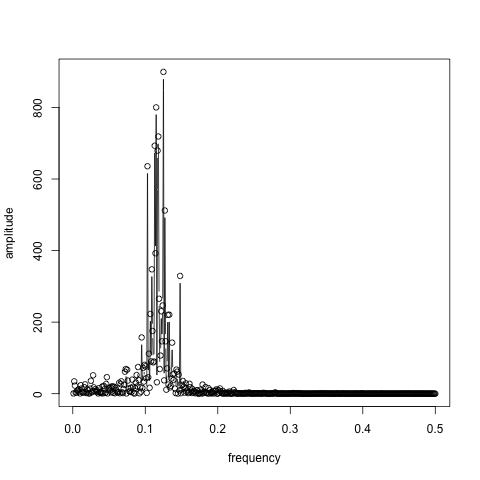
\includegraphics[width=4in]{../code/periodogram1000} 
   \caption{periodogram for 1000 obervation}
   \label{fig:periodogram1000}
\end{figure}
Smooth peridogram
\begin{figure}[H] %  figure placement: here, top, bottom, or page
   \centering
   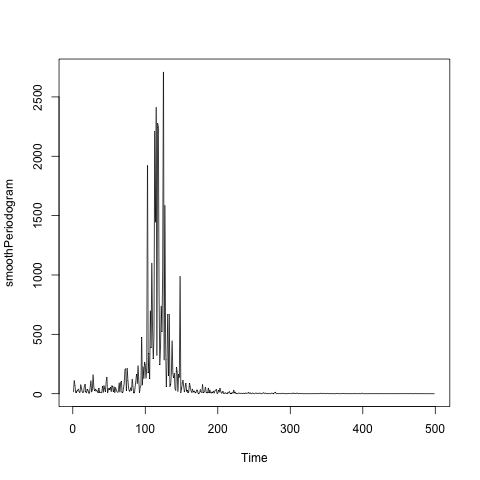
\includegraphics[width=4in]{../code/smoothPeriodogram1000.png} 
   \caption{Smoother periodogram}
   \label{fig:smoothp}
\end{figure}

Estimated spectral density
\begin{figure}[H] %  figure placement: here, top, bottom, or page
   \centering
   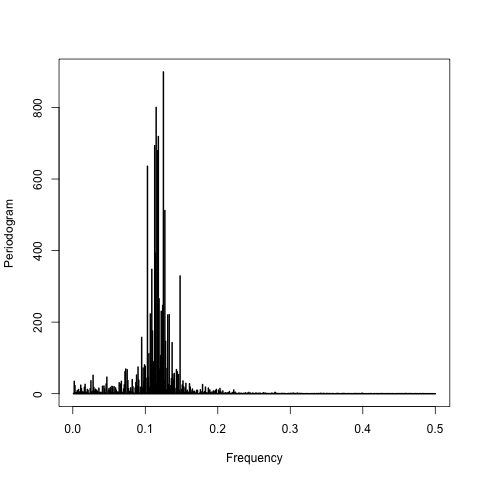
\includegraphics[width=4in]{../code/estimatedSpecralDensity1000.png} 
   \caption{Estimated spectral density}
   \label{fig:es1000}
\end{figure}
\justify
For 1000 observations, the the peak is at at frequency of 0.125 corresponding to 8 time periods

\section{Problem 8.3}
If the process $\{X_{t} \}$ is a causal ARMA(p,q), its spectral density is given by \cite{petter}
\begin{equation}
f_{X}(\lambda) = \frac{\sigma^{2}}{2\pi}\frac{| \theta(e^{-i\lambda}) |^{2}}{| \phi(e^{-i\lambda}) |^{2}}, \quad -\pi \leq \lambda \leq \pi.
\end{equation}
Furthermore, 
\begin{equation}
\begin{split}
 \theta(e^{-i\lambda})  &= 1+\theta_{1}e^{-i\lambda} + \theta_{2}e^{-i2\lambda} + \cdots +\theta_{n}e^{-in\lambda}\\
 			          &=1+\sum_{k=0}^{n}\theta_{n}e^{-ik\lambda},
  \end{split}
\end{equation}
and 
\begin{equation}
\begin{split}
 \phi(e^{-i\lambda})  &= 1-\phi_{1}e^{-i\lambda} - \phi_{2}e^{-i2\lambda} - \cdots -\phi_{n}e^{-in\lambda}\\
                                &=1-\sum_{k=0}^{n}\phi_{n}e^{-ik\lambda}
 \end{split}
\end{equation}
where 
\begin{equation}
e^{-ik\lambda} = \cos(k\lambda) - i\sin(k\lambda).
\end{equation}
Now let 
\begin{equation}
\begin{split}
f(\lambda)  &= e^{-ik\lambda} \\
                  &= \cos(k\lambda) - i\sin(k\lambda),
 \end{split}
\end{equation}
and let $\lambda_{0}$ be arbitrary taken from the interval $[-\pi, \pi]$. Then 
\begin{equation}
\begin{split}
\lim_{\lambda\to\lambda_{0}}f(\lambda) &= \lim_{\lambda\to\lambda_{0}}\cos(k\lambda) - i\sin(k\lambda)\\
&=cos(k\lambda_{0}) - i\sin(k\lambda_{0})\\
&=f(\lambda_{0})
\end{split}
\end{equation}
and this prove that $e^{-ik\lambda}$ is continuous and so is its linear combination
\begin{equation}
\theta(e^{-ik\lambda}) = 1+\sum_{k=0}^{n}\theta_{n}e^{-ik\lambda}  \nonumber
\end{equation}
and
\begin{equation}
\phi(e^{-ik\lambda}) = 1-\sum_{k=0}^{n}\phi_{n}e^{-ik\lambda}.  \nonumber
\end{equation}
Since we have a causal process, the roots of $\phi(e^{-ik\lambda})$ lies outside the unit circle, and $\phi(e^{-ik\lambda}) \neq 0$, and since 
the quotient of two continuous functions is continuous we have that
\begin{equation}
\frac{\theta(e^{-i\lambda}) }{\phi(e^{-i\lambda}) }  \nonumber
\end{equation}
is continuous
and 
\begin{equation}
\frac{| \theta(e^{-i\lambda}) |^{2}}{| \phi(e^{-i\lambda}) |^{2}}  \nonumber
\end{equation}
is also continuous. Therefore 
\begin{equation}
f_{X}(\lambda) = \frac{\sigma^{2}}{2\pi}\frac{| \theta(e^{-i\lambda}) |^{2}}{| \phi(e^{-i\lambda}) |^{2}}, \quad -\pi \leq \lambda \leq \pi.  \nonumber
\end{equation}
is continuous.
\justify
Assume now that the minimum of the spectral density is attained at some value, say $\lambda_{0}$. Then the minimum of the spectral density is 
\begin{equation}
\begin{split}
f_{X}(\lambda_{0}) &= \frac{\sigma^{2}}{2\pi}\frac{| \theta(e^{-i\lambda_{0}}) |^{2}}{| \phi(e^{-i\lambda_{0}}) |^{2}}, \quad -\pi \leq \lambda \leq \pi.\\
&=\frac{\sigma^{2}}{2\pi}\left|\frac{ \theta(e^{-i\lambda_{0}}) }{ \phi(e^{-i\lambda_{0}})}\right|^{2} \\
&=\frac{\sigma^{2}}{2\pi}\left|\frac{ 1+\sum_{k=0}^{n}\theta_{k}e^{-ik\lambda}}{ 1-\sum_{k=0}^{n}\phi_{k}e^{-ik\lambda}}\right|^{2} \geq 0.  \nonumber
\end{split}
\end{equation}
For $f_{X}(\lambda_{0})$ to be equal to zero, we need 
\begin{equation}
1+\sum_{k=0}^{n}\theta_{k}e^{-ik\lambda} = 1+ \sum_{k=0}^{n}\theta_{k}\cos(k\lambda) + i\sum_{k=0}^{n}\theta_{k}\sin(k\lambda) = 0.  \nonumber
\end{equation}
This mean that we need to have simultaneously 
\begin{equation}
\sum_{k=0}^{n}\theta_{k}\sin(k\lambda) = 0.  \nonumber
\end{equation}
and 
\begin{equation}
 \sum_{k=0}^{n}\theta_{k}\cos(k\lambda)  = -1.  \nonumber
\end{equation}
\justify
Furthermore,
\begin{equation}
\sum_{k=0}^{n}\theta_{k}\sin(k\lambda) = 0,  \nonumber
\end{equation}
means that 
either $\theta_{k} = 0$ or $\sin(k\lambda) = 0$, $\forall k=1, \cdots, n$. Since all $\theta_{k}$ can not be equal to zero, the latter must hold, that is 
\begin{equation}
\begin{split}
\sin(\lambda) &= 0\\
\sin(2\lambda) &= 0\\
&\vdots\\
\sin(n\lambda) &= 0\\  \nonumber
\end{split}
\end{equation}
which means that 
\begin{equation}
n\lambda = \pm\frac{\pi}{2} \Rightarrow \lambda = \pm\frac{\pi}{2n} .
\end{equation}
Similarely,
\begin{equation}
 \sum_{k=0}^{n}\theta_{k}\cos(k\lambda)  = -1.  \nonumber
\end{equation}
means that at $\lambda = \pm\frac{\pi}{2n}$ we must have
\begin{equation}
\theta_{1}\cos\left(\frac{\pi}{2}\right) + \theta_{2}\cos\left(2\frac{\pi}{4}\right)+\cdots + \theta_{n}\cos\left(n\frac{\pi}{2n}\right) = -1\nonumber,
\end{equation}
but 
\begin{equation}
\theta_{1}\cos\left(\frac{\pi}{2}\right) + \theta_{2}\cos\left(2\frac{\pi}{4}\right)+\cdots + \theta_{n}\cos\left(n\frac{\pi}{2n}\right) = 0 \nonumber
\end{equation}
so 
\begin{equation}
\theta_{1}\cos\left(\frac{\pi}{2}\right) + \theta_{2}\cos\left(2\frac{\pi}{4}\right)+\cdots + \theta_{n}\cos\left(n\frac{\pi}{2n}\right) \neq -1\nonumber
\end{equation}
Therefore 
\begin{equation}
f_{X}(\lambda_{0}) = \frac{\sigma^{2}}{2\pi}\left|\frac{ 1+\sum_{k=0}^{n}\theta_{k}e^{-ik\lambda}}{ 1-\sum_{k=0}^{n}\phi_{k}e^{-ik\lambda}}\right|^{2} > 0.  \nonumber
\end{equation}








\section{Problem 8.4}

Let $\{ X_{t}, t = 1, \cdots, n \}$ be a data from a time series
The likelihood estimator of the autocovariance function $\Gamma_{LM}$ is given by \cite{petter}
\begin{equation}
\Gamma_{LM} = (2\pi)^{-n/2}(det(\Gamma_{n}))^{-1/2}\exp\left(  -\frac{1}{2}\mathbb(X^{\prime}\Gamma_{n}^{-1}\mathbb(X_{n})) \right)
\end{equation}
and the sample autocovariance is given by
\begin{equation}
\hat{\Gamma}_{n} = 
\begin{bmatrix}
    \hat{\gamma}(0) & \hat{\gamma}(1)  & \dots  & \hat{\gamma}(k-1) \\
        \hat{\gamma}(1) & \hat{\gamma}(0) & \dots  & \hat{\gamma}(k-2) \\
    \vdots & \vdots & \vdots & \vdots \\
        \hat{\gamma}(k-1) & \hat{\gamma}(k-2)  & \dots  & \hat{\gamma}(0)
\end{bmatrix}
\end{equation}
where 
\begin{equation}
\hat{\gamma}(h) = \frac{1}{n}\sum_{t=1}^{n-|h|}(X_{t+|h|}-\bar{X})(X_{t}-\bar{X})
\end{equation}







\section{Problem 8.5}
Let $\{ X_{t}, t = 1, \cdots, n \}$ be a data from a time series. Supposed that we fit the AR(p) process to the data using the Yule Walker estimation of $\phi$ and $\sigma^{2}$.
Let explain $\hat{\Gamma_{YW}}(h) = \hat{\gamma}(h)$ for $|h|\leq p$.
\justify
 From \cite{petter}, the Yule-Walker estimators $\hat{\phi}$ and $\hat{\sigma}^{2}$ of $\phi$ and $\sigma^{2}$ are solutions of
\clearpage
\begin{equation}\label{eq:gam}
\hat{\Gamma}_{p}\hat{\phi} = \hat{\gamma}_{p}
\end{equation}
and
\begin{equation}\label{eq:sig}
\hat{\sigma}^{2} = \hat{\gamma}(0)- \hat{\phi^{\prime}}\hat{\gamma}_{p}
\end{equation}
respectively. Where
\begin{equation}\label{eq:auto}
\hat{\Gamma}_{p} = [\hat{\gamma}(i-j)]_{i,j=1}^{p},
\end{equation}
and
\begin{equation}
\hat{\gamma}_{p} = (\hat{\gamma}(0), \cdots , \hat{\gamma}(p).
\end{equation}
For every nonsingular covariance matrix of the form (\ref{eq:auto}), there is an AR(p) process whose autocovariance at lages $0, \cdots, p$ are $\gamma(0),\cdots,\gamma(p)$ where the coefficients and white noise are computed from the sample Yule-Walker equations \cite{petter}. Consequently, from \cite{petter} the Solutions of (\ref{eq:gam}) and (\ref{eq:sig}) is 
\begin{equation}
\gamma_{F}(h) = \hat{\gamma}(h), \quad, h=0,\cdots, p
\end{equation}
Which are found from the Durbin-Levinson algorithm \cite{petter}. Therefore the autocovariance of the fitted model at lags $0, \cdots, p$ coincide with that of the sample autocovariance \cite{petter} 



\section{Problem 8.6}
Let $\{ X_{t}, \}$ be a MA(2) process
\begin{equation}
X_{t} = \theta(B)Z_{t} = (1-B\xi_{1}^{-1})(1-B\xi_{2}^{-1})Z_{t}, \quad \{ Z_{t}, \} \sim WN(0, \sigma^{2})
\end{equation}

\subsection{Part a}
\begin{equation}
X_{t} = \theta_{1}Z_{t-1} + \theta_{2}Z_{t-2} + Z_{t}
\end{equation}
For an ARMA(p,q) process we  have
\begin{equation}\label{eq:armapq}
\hat{\gamma}(k)-\phi_{1}\hat{\gamma}(k-1)-\cdots-\phi_{p}\hat{\gamma}(k-p) = \sigma^{2}\sum_{j=k}^{q}\theta_{j}\psi_{j-k}, \quad 0 \leq k \leq p+q.
\end{equation}
For an MA(2) process equation (\ref{eq:armapq}) reduces to 
\begin{equation}\label{eq:maq}
\hat{\gamma}(k) = \sigma^{2}\sum_{j=k}^{2}\theta_{j}\psi_{j-k}, \quad 0 \leq k \leq 2.
\end{equation}
or
\begin{equation}\label{eq:maq1}
\hat{\gamma}(0) = \sigma^{2}(1+ \theta_{1}\psi_{1} + \theta_{2}\psi_{2})
\end{equation}
\begin{equation}\label{eq:maq2}
\hat{\gamma}(1) = \sigma^{2}( \theta_{1} + \theta_{2}\psi_{1})
\end{equation}
\begin{equation}\label{eq:maq3}
\hat{\gamma}(2) = \sigma^{2} \theta_{2}
\end{equation}
from which $\theta_{1}, \theta_{2}$ can be computed from

\subsection{Part b}
The coefficient $\{\tilde{\theta}_{j}, j=1,2\}$ Applying the Durbin-Levinson algorithm to the sample autocovariance we can fit the MA(2) process \cite{petter}. The model then becomes
\begin{equation}
X_{t} = \hat{\theta}_{21}Z_{t-1} +  \hat{\theta}_{22}Z_{t-2} + Z_{t}
\end{equation}

\subsection{Partc}
Finding the filter that fits 
\begin{equation}
X_{t} = \tilde{\theta}(B)\tilde{Z}_{t}
\end{equation}

%%%%%%%%%%%%%%%%%%%%%%%%%%%%%%%%%%%%%%%%%%%%%
%%%%%%%%%%%%%%%%%%%%%%%%%%%%%%%%%%%%%%%%%%%%%
%%%%%%%%%%%%%%%%%%%%%%%%%%%%%%%%%%%%%%%%%%%%%
%%%%%%%%%%%%%%%%%%%%%%%%%%%%%%%%%%%%%%%%%%%%%
\begin{thebibliography}{9}
\bibitem{petter} 
Petter J. Brockwell. Richard A. Davis
\textit{Introduction to Time Series and Forecasting}. 
Springer. Second edition. 2001

\bibitem{penn} 
PennState Eberly College of science, 
\textit{STAT 510. Applied Time Series Analysis}. 
https://newonlinecourses.science.psu.edu/stat510/node/71/
 
\end{thebibliography}


\end{document}  